\documentclass[preprint,12pt]{elsarticle}
\usepackage[UTF8,scheme=plain,fontset=fandol]{ctex}
\usepackage{amsmath,amssymb,bm}
\usepackage{booktabs,multirow,threeparttable}
\usepackage{graphicx,subcaption}
\usepackage{siunitx}
\usepackage{xcolor,hyperref,lineno,enumitem}
\usepackage{placeins}
\graphicspath{{../figures/}}
\hypersetup{colorlinks=true,linkcolor=blue!50!black,citecolor=blue!50!black,urlcolor=blue!60!black}
\emergencystretch=2em
\journal{Transportation Research Part C}
\renewcommand{\figurename}{图}
\renewcommand{\tablename}{表}

\begin{document}
\begin{frontmatter}

\title{面向全生命周期成本与油电混行能耗的高速公路三维线形数据驱动协同优化}

\author[aff1]{匿名作者}
\affiliation[aff1]{organization={双盲审稿匿名单位},city={匿名},country={中国}}

\begin{abstract}
高速公路线形同时耦合平面几何、纵断面、地形、桥隧、城市建设强度与长期车辆运行。本文构建数据驱动双目标框架，将准天然数字高程模型（DEM）、OpenStreetMap（OSM）交通/水系/建筑图层和14,018个GNSS点融合至统一数字走廊，以50个低频平面模态和224个活跃坡段变量协同描述三维线形。全生命周期成本包含占地、基本工程、结构、土方和养护；第二目标将30年油电混行车流的燃油与电耗货币化。候选线形与OSM障碍物相交时触发跨越桥，连通山体触发生态隧道，高密度建成区核心禁行。IJS用于加权和前沿近似，所得候选依次通过硬可行、预算、非支配与熵权折中筛选。

模型应用于广州北环高速浔峰洲—黄村段（22.46 km）。在端点高程锚定、谱宽参数$W=500$ m且密度约束开启时，折中方案将全生命周期成本由26.4061亿元降至24.2078亿元（$-8.33\%$），将货币化车流能耗由13.9460亿元降至13.5278亿元（$-3.00\%$）；最小半径421 m、硬罚为0、Tier-2穿越为0，Tier-1由2.010 km降至1.591 km。线路增加12 m且土方上升，但结构费降低2.37亿元，表明收益来自可追踪的物理权衡而非缩短里程。旧自由端点、不等预算实验仅作探索性证据；设计级使用前仍需完成当前模型多种子、等NFE复现。
\end{abstract}

\begin{keyword}
高速公路线形优化 \sep 数字高程模型 \sep OpenStreetMap \sep 改进水母搜索算法 \sep 全生命周期成本 \sep 油电混行能耗 \sep 平纵协同
\end{keyword}
\end{frontmatter}

\linenumbers

\section{引言}

高速公路线形一旦在前期确定，将长期影响建设投资、桥隧比例、土石方调配、养护暴露和车辆运行。一条线位的微小横移会改变其所穿越的地面高程、障碍物和建筑区；平面路径缩短可能造成纵断面恶化；绕避山体可能进入高密度建成区；降低土方可能需要增设桥梁；未经端点控制的纵断面还可能利用“起高终低”获得虚假节能。因此，线形优化的核心不是单独拟合一条曲线，而是在空间数据、工程规范和竞争目标共同作用下寻找可实施的三维方案。

早期研究已证明平面与纵断面同步优化的必要性\cite{chew1989,jong2003}。此后，研究者发展了走廊带模型、混合整数方法、环境目标和偏好驱动的多目标搜索\cite{kang2012,mondal2015,hirpa2016,vazquez2018,akhmet2022}；近年又引入BIM、GIS、深度强化学习、采样式路径规划及强化学习—群智能混合搜索\cite{han2023,he2023,alhadad2024,pu2024,pu2026}。然而，现有综述仍指出算法模型与真实工程异构约束之间存在明显鸿沟\cite{songreview2023}。

本文针对三类问题展开改进。第一，单一中线高程或理想化地价栅格不能使平面横移真正改变地形，从模型结构上削弱平纵协同。第二，固定桥隧长度和不连续惩罚会给优化器留下“利用计价规则”的空间。第三，高维非线性搜索容易把局部曲率、坡差等违约平均掉，产生目标低而不可行的解。

本文以林坤锐学位论文\cite{lin2025}的全生命周期成本—能耗数学模型为基底，将其以NSGA-II和单中线数据为主的实现扩展为当前数据驱动实验。主要贡献如下：

\begin{enumerate}[leftmargin=*,label=(\arabic*)]
\item 建立GNSS、准天然DEM、OSM交通/水系和建筑密度三级区共同驱动的数字走廊；
\item 建立桥梁交叉触发、生态隧道、土方—结构替代以及接线端点高程内生于三维几何的工程化全生命周期模型；
\item 构建名义275槽、实际274个活跃变量的平纵协同参数化，并实现成本—油电混行能耗双目标决策；
\item 提出经数值修正的IJS，将独立Tent初始化、L\'evy探索与DE精修结合；
\item 建立可审计证据链，明确区分当前工程结果与模型开发早期的探索性实验。
\end{enumerate}

图\ref{fig:overview_zh}展示从数据到可行线形的完整流程。图中每个模块均对应仓库中的可复核数据、模型或结果文件。

\begin{figure*}[t]
\centering
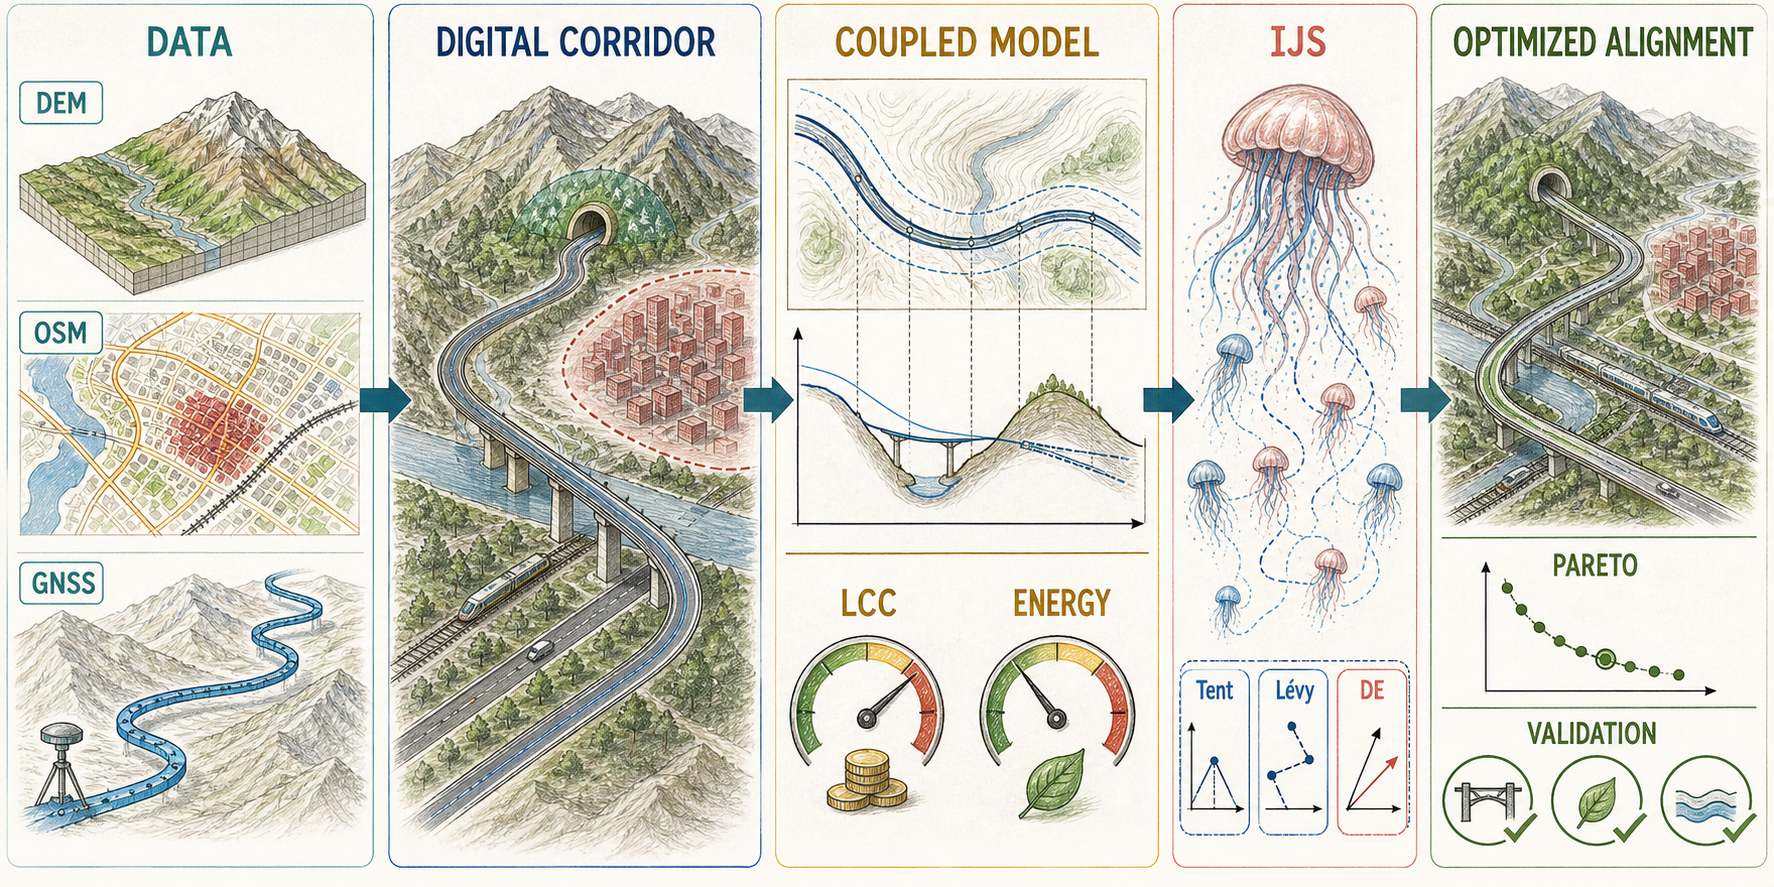
\includegraphics[width=\textwidth]{method_overview_handdrawn.png}
\caption{高速公路三维线形数据驱动协同优化方法总览。手绘科研图用于表达信息流，数学定义见第3、4节。}
\label{fig:overview_zh}
\end{figure*}

\section{相关研究}

\subsection{三维线形与空间数据}

Chew等\cite{chew1989}较早建立平纵同步优化模型，Jong和Schonfeld\cite{jong2003}进一步采用进化编码处理三维非凸搜索。此后，GIS环境约束、指定走廊平面优化和双目标三维线形得到发展\cite{kang2012,mondal2015,hirpa2016}。V\'azquez-M\'endez等\cite{vazquez2018}将基础设施成本纳入三维模型，Akhmet等\cite{akhmet2022}对公路纵断面双目标问题进行更严格求解。BIM端到端设计、低碳强化学习、3D-RRT*及策略优化—群智能混合方法进一步提升了自动化程度\cite{han2023,he2023,pu2024,pu2026}。这些研究表明，算法进步必须与可解释的地形—结构—规范映射同时推进。

\subsection{全生命周期成本与车流能耗}

本文沿用学位论文\cite{lin2025}的占地、桥隧、基本建设、养护和土方费用体系，并将其重新映射到候选三维线形。线形一致性会显著影响车辆排放\cite{llopis2019}；电动车能耗又受到纵坡、质量、附属能耗和再生制动的共同影响\cite{dimartino2022}。为避免直接相加升、千瓦时等不相容量纲，本文在30年分析期内将油耗和电耗货币化，但保留燃油与电动两类分项，避免把货币指标误写为唯一环境指标。

\subsection{算法与多目标决策}

NSGA-II是常用多目标基准\cite{deb2002}，但高维纵断面变量会显著增加进化搜索负担。JS模拟水母随洋流运动及主动/被动运动\cite{chou2021}。本文在JS上增加Tent、L\'evy和DE\cite{storn1997}，并通过消融判断各组件是否真正有效。熵权法以Shannon信息量为基础\cite{shannon1948}；本文先进行硬可行、预算和非支配筛选，再在剩余前沿中定权选点，从程序上禁止“权重抵消违约”。

\section{数据驱动数学模型}

\subsection{工程案例与数据融合}

案例为广州北环高速浔峰洲—黄村段，双向六车道，实测中线长22.462 km。14,018个GNSS点提供平面坐标、高程、现状方案M-A、固定平面端点和接线高程。

地形来自AWS Terrain Tiles\cite{awsterrain}的60幅z14瓦片，像元约8.8 m。由于该DEM反映现状地表，模型先掩膜实测中线两侧60 m道路影响带，再以邻域插值重建“准天然地面”，并进行1.57 m垂直基准校正；与实测中线高程的相关系数为0.915。该方法不能替代建路前测量，但保证M-A与候选方案采用同一土方口径。

OSM\cite{haklay2008,osmlicense}提供道路、铁路、水系和建筑轮廓。剔除北环自身及伴行线后，障碍物包括4,807条道路、857条铁路和338条河流/运河。建筑轮廓在25 m网格上栅格化，并以200 m尺度平滑；阈值按现状线所能穿越的最大密度标定，形成Tier 2硬禁行、Tier 1可穿越但抑制、Tier 0自由三类。图\ref{fig:case_zh}给出多源数据在局部工程坐标系中的叠加关系。

\begin{figure*}[t]
\centering
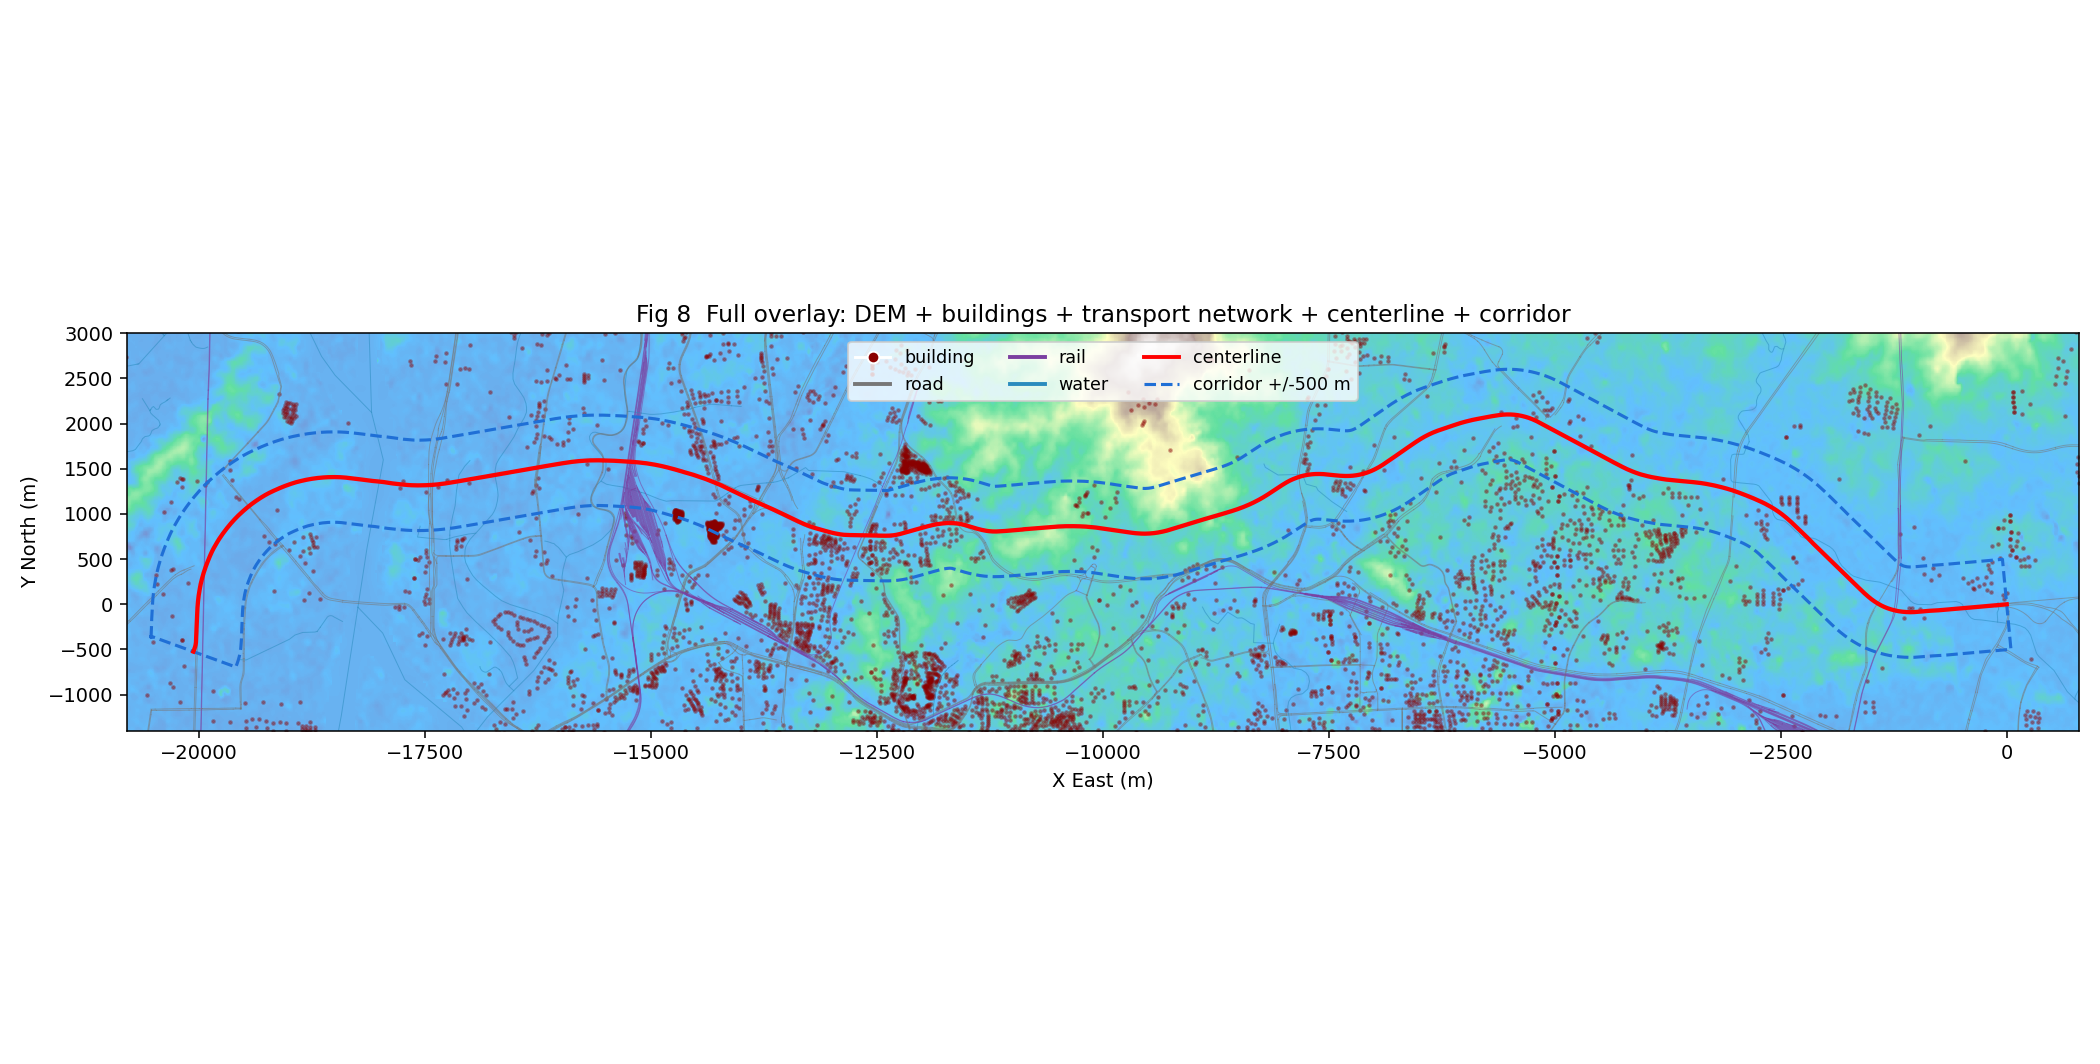
\includegraphics[width=\textwidth]{case_data_layers.png}
\caption{案例区DEM、OSM建筑/道路/铁路/水系、实测中线及用于空间参照的$\pm500$ m带。优化器中的$W$是一阶正弦模态幅值，并非逐点硬偏移边界。}
\label{fig:case_zh}
\end{figure*}

\subsection{平纵协同决策变量}

设实测平面线为$\bm r_0(s)=[x_0(s),y_0(s)]^\top$，单位法向为$\bm n(s)$。候选平面以法向偏移表示：
\begin{equation}
\delta(s)=\sum_{k=1}^{50}a_k\sin\left(\frac{k\pi s}{L_0}\right),\qquad
|a_k|\leq \frac{W}{k^2},
\label{eq:sine_zh}
\end{equation}
主实验$W=500$ m，$\bm r(s)=\bm r_0(s)+\delta(s)\bm n(s)$。正弦基固定起终点，并给出保守谱包络$|\delta|\leq W\sum_{k=1}^{50}k^{-2}\approx1.625W$，故$W$不是逐点硬边界；当前M-C最大采样偏移约184 m。三次样条重建后，曲率与半径为
\begin{equation}
\kappa(s)=\frac{|x'y''-y'x''|}{(x'^2+y'^2)^{3/2}},\qquad R(s)=\kappa(s)^{-1},
\end{equation}
所有目标与约束在约10 m桩号网格上计算。

纵断面采用225个变坡控制量，间距约100 m。为固定首末接线高程，令原始坡度扰动$h_i\in[-1,1]$、坡段长$\Delta s_i$、最大纵坡$g_{\max}=0.04$，则
\begin{align}
\bar h&=\frac{\sum_i h_i\Delta s_i}{\sum_i\Delta s_i},\qquad
g_{\mathrm{req}}=\frac{z_L-z_0}{\sum_i\Delta s_i},\\
g_i&=g_{\mathrm{req}}+\lambda g_{\max}(h_i-\bar h),
\label{eq:grade_zh}
\end{align}
其中$\lambda$取保证$|g_i|\leq g_{\max}$的最大缩放值。因此$\sum_i g_i\Delta s_i=z_L-z_0$恒成立，优化器无法通过整体下倾获取虚假节能。实现仍保留225槽纵断面块，其中端点锚定时起点高程槽被忽略，故存储向量为275槽、实际活跃变量为274个（50个模态和224个坡段）；约150个平面重建控制点不属于决策变量。

\subsection{全生命周期成本目标}

成本目标为
\begin{equation}
\min C=C_R+C_B+C_S+C_Q+C_{TU},
\end{equation}
分别对应占地、桥隧、基本工程、折现养护和土方调运。实现中的主要分项为
\begin{align}
C_R&=c_{land}\frac{LB}{666.67}+5000\frac{L}{1000},\\
C_B&=c_BL_B+C_{ramp}+c_TL_T,\qquad C_S=(c_{sg}+c_{pv})L,\\
C_Q&=\sum_{y=1}^{T}\frac{1}{(1+r)^y}\sum_i\Delta s_i
[\gamma+365Q_y\tau+c_{soil}\Phi_i].
\end{align}
结构豁免段$\Phi_i=0$。单价基于学位论文及《广州市本级政府投资项目估算编制指引（2025版）》\cite{guangzhou2025}，分析期30年、折现率5\%。

设桩号$j$的设计—地面高差为$h_j=z_j-z^g_j$、路基宽度为$B$、边坡率系数为$m$，断面面积近似为
\begin{equation}
A_j=B|h_j|+mh_j^2.
\end{equation}
土方体积与费用采用
\begin{equation}
V^{\pm}=\sum_j\frac{A_j^{\pm}+A_{j+1}^{\pm}}{2}\Delta s_j,\qquad
C_{TU}=E_L+\sum_j\Delta s_j\min(c_{ew}A_j,c_{str}).
\end{equation}
当填/挖单价超过桥/隧单价，或高填深挖超过30 m时触发结构替代；结构区土方豁免，从而避免重复计价和“悬浮免费”退化解。

候选线形与OSM主干道路、铁路或水系相交时触发跨越桥。若障碍宽度为$b_q$、交角为$\theta_q$，桥区长度为
\begin{equation}
\ell_q=\frac{b_q}{\max(\sin\theta_q,\sin15^\circ)}+2E_{\mathrm{ext}},
\end{equation}
其中$E_{\mathrm{ext}}=75$ m，相邻间隙小于100 m则合并。七座既有立交的匝道功能费以现状校准常数计，主线桥长度则由几何内生。DEM中高程不低于70 m的连通山体经500 m闭运算形成白云山生态强制隧道区；其面积19.2 km$^2$、M-A穿越1.28 km，与独立资料约21 km$^2$、1.35 km接近。

\begin{table}[t]
\centering
\caption{案例当前模型主要参数。}
\resizebox{\linewidth}{!}{\begin{tabular}{lll}
\toprule
类别 & 参数 & 数值 \\
\midrule
几何 & 速度/宽度/$R_{min}$/$g_{max}$ & 100 km/h/25.5 m/400 m/4\% \\
寿命期 & 年限/折现率 & 30年/5\% \\
占地与基本工程 & 地价/路基/路面 & 58,641元/亩；200/30,000元/m \\
桥隧 & 桥/隧/$E_{ext}$ & 1.56/2.70亿元/km；75 m \\
土方 & 挖/填/边坡率 & 30/25元/m$^3$；1:1.5 \\
交通 & AADT/电动车占比 & 30,000辆/日；0.30 \\
能源 & 油价/电价 & 8元/L；0.8元/kWh \\
搜索 & 种群/迭代/权重点 & 200/1,000/21 \\
\bottomrule
\end{tabular}}
\end{table}

\subsection{油电混行能耗目标}

30年货币化能耗为
\begin{equation}
\min E=\sum_{y=1}^{30}\frac{365Q_y}{(1+r)^y}
\left[(1-p_{EV})c_fe_f(\bm x)+p_{EV}c_ee_e(\bm x)\right],
\end{equation}
其中基准AADT为30,000辆/日，$p_{EV}=0.30$，油价8元/L、电价0.8元/kWh。燃油车受空气、滚动、坡度和残余横向阻力共同作用：
\begin{align}
F_{air}&=\tfrac12\rho C_dA_fv^2, & F_r&=C_rm_vg\cos\alpha,\\
F_g&=m_vg\sin\alpha, &
F_a&=\max\left(0,\frac{m_vv^2/R-m_vgS_p}{N_vC_s}\right).
\end{align}
燃油车外部功率与单车单程油耗为
\begin{align}
P_{ex,i}&=\max\left(0,\frac{(F_{air}+F_r+F_g+F_a)v}{736\eta_f}\right),\\
e_f(\bm x)&=\sum_i\phi(HP_{in}+P_{ex,i})\frac{\Delta s_i}{v}/1000,
\end{align}
其中$\phi=0.03$ ml/(s hp)、$HP_{in}=27$ hp、$\eta_f=0.85$。原论文式(4.12)末尾的$10^{-3}$会使横向阻力低约五个数量级，故代码按量纲校核删除该项并显式声明。电动车令$W_i=(F_{air}+F_r+F_g+F_a)\Delta s_i$，则
\begin{equation}
e_e=\frac{1}{3.6\times10^6}\sum_i
\begin{cases}W_i/\eta_e,&W_i\geq0,\\W_i\eta_e,&W_i<0,\end{cases}
+0.15L_{km},\qquad\eta_e=0.90\times0.95.
\end{equation}
当前主实验计算代表方向，端点锚定消除了净落差套利；双向平均仍待完善。

\subsection{约束与折中决策}

硬约束包括平纵端点固定、$R(s)\geq400$ m、$|g_i|\leq4\%$、$|g_{i+1}-g_i|\leq3\times10^{-4}\Delta s_{ctrl}$、交叉角不小于$15^\circ$以及Tier 2穿越为0；规范值来自JTG D20—2017\cite{jtgd20}。$W$控制模态幅值而非逐点硬约束，当前线仍在图示$\pm500$ m参照带内。令$H(\bm v)=\mathrm{mean}(\bm v)+\max(\bm v)$，惩罚为
\begin{equation}
P=\rho_t[30H(\bm v_R)+10H(\bm v_{\Delta g})+10H(\bm v_{skew})+10H(\bm v_{D2})],
\end{equation}
其中$v_R=[400-R]_+/400$，$v_{D2}=\min(d_{D2}/100,5)$，前/后半程$\rho_t=0.3/3.0$；Tier 1不进入硬罚。

同一基准种群产生$C_{ref},E_{ref}$和熵权$w_C,w_E$，标量目标为
\begin{equation}
F(\bm x)=w_C\frac{C}{C_{ref}}+w_E\frac{E}{E_{ref}}+P(\bm x)
+0.22\frac{L_{T1}}{L}.
\end{equation}
对$n\times2$指标矩阵，极差归一化$z_{ij}$后取$p_{ij}=z_{ij}/\sum_i z_{ij}$、$e_j=-(\ln n)^{-1}\sum_i p_{ij}\ln(p_{ij}+10^{-12})$、$w_j=(1-e_j)/\sum_k(1-e_k)$。初始种群熵权用于搜索标量化，存活前沿上重新计算的熵权用于最终折中，二者不是同一次定权。21个加权和问题只构成Pareto近似，可能遗漏非凸前沿的非支撑点。之后依次执行硬可行、规划假设预算$C\leq1.1C_{M-A}$、非支配和前沿熵权筛选；10\%预算容差不是法定阈值，仍需敏感性检验。

\section{改进水母搜索算法}

\subsection{算法机制}

原始JS在洋流运动与种群内主动/被动运动之间切换\cite{chou2021}。本文IJS进行三项改进：
\begin{itemize}[leftmargin=*]
\item \textbf{独立Tent初始化：}每个个体使用独立混沌链且$\mu=1.99$；避免$\mu=2$在float64中塌缩为0，也避免单链造成个体相关。
\item \textbf{搜索域缩放L\'evy飞行：}步长乘$0.01(\bm u-\bm l)$；原未缩放实现的接受率仅0.48\%。
\item \textbf{DE精修：}以种群差分构造变异和交叉向量（$CR=0.5$），并采用精英接受\cite{storn1997}。
\end{itemize}

时间控制为$A_r=(1-t/T)(2u-1)$。$|A_r|\geq0.5$时，主试探为$\bm x_i+\bm u\odot(\bm x_{best}-3u\bar{\bm x})$；否则执行朝优质随机同伴的主动运动或$\bm x_i+0.1\bm u\odot(\bm u_b-\bm l_b)$被动运动。L\'evy试探为$\bm x_i^L=\bm x_i+\bm u\odot[0.01(\bm u_b-\bm l_b)\odot\bm L_{1.5}]$；DE采用$\bm m_i=\bm x_i+u(\bm x_{r1}-\bm x_{r2})$、$CR=0.5$二项交叉与贪婪替换。越界分量先跨对侧边界反射再截断。

因此IJS每代约包含3倍种群评价量，本文同时报告NFE/时间，避免把同代数误认为同预算。惩罚采用前半程0.3倍、后半程3倍的两阶段调度。图\ref{fig:flow_zh}给出算法闭环。

\begin{figure}[t]
\centering

\includegraphics[height=.72\textheight,keepaspectratio]{ijs_flowchart_handdrawn.png}
\caption{IJS算法流程。每个算子后均精英接受；停止后进行Pareto筛选与熵权折中，而非几何膝点选择。}
\label{fig:flow_zh}
\end{figure}
\FloatBarrier

\subsection{实验协议}

主方案采用种群200、迭代1,000、21个权重点，目标与约束在10 m网格评价。历史消融固定实测平面并采用名义225维自由高程模型，五个变体各30次、种群200、迭代500；历史多算法实验在95--500个存储变量上比较六种算法，每个组合10次。原表$p$值来自独立样本Mann--Whitney/秩和检验，不是配对符号秩检验。两组实验均早于端点锚定与密度分区；相同代数也不代表相同NFE：500代时JS、单附加算子和完整IJS约为100,200、200,200和300,400次求值。因此这些实验仅作为透明的开发证据，不能证明当前模型下IJS的等预算优越性；237点历史敏感性也采用同一效度边界。

\section{实验结果}

\subsection{当前工程方案}

表\ref{tab:current_zh}与图\ref{fig:scheme_zh}为当前主结果。M-C使$C$降低8.33\%、$E$降低3.00\%。线长增加12 m（+0.05\%），说明收益并非来自人为缩短线路；桥隧费减少2.37亿元，而土方费增加0.15亿元。其工程含义是：优化器接受了略长线路和更多土方，以换取更低结构暴露和运行能耗。

边坡诊断量$Q=\sum_{u=1}^{5}W_uS_u$，评分$S_u\in\{1,3,5\}$，地形、沟壑、降雨、地质、植被权重为$(0.30,0.15,0.20,0.20,0.15)$。地形评分取纵坡角与填挖高度分级的较大者，其余四项为走廊级标定常数。因此$Q$仅是比较筛查指标，不是失稳概率模型，也不进入优化目标。

\begin{table}[t]
\centering
\caption{当前端点锚定、建筑密度约束开启的方案对比。}
\label{tab:current_zh}
\begin{tabular}{lrrr}
\toprule
指标 & M-A现状 & M-C优化 & 变化 \\
\midrule
全生命周期成本（亿元） & 26.4061 & 24.2078 & $-8.33\%$ \\
车流能耗（亿元） & 13.9460 & 13.5278 & $-3.00\%$ \\
\quad 燃油分项 & 11.1072 & 10.7911 & $-2.85\%$ \\
\quad 电耗分项 & 2.8388 & 2.7367 & $-3.60\%$ \\
里程（km） & 22.4618 & 22.4741 & $+0.05\%$ \\
最小平曲线半径（m） & 422 & 421 & 合规 \\
边坡危险度 & 3.309 & 3.298 & $-0.35\%$ \\
Tier-1穿越（km） & 2.010 & 1.591 & $-20.85\%$ \\
Tier-2穿越（km） & 0 & 0 & 合规 \\
硬约束罚值 & 0 & 0 & 合规 \\
\bottomrule
\end{tabular}
\end{table}

\begin{figure*}[t]
\centering

\includegraphics[width=\textwidth]{current_scheme_summary.pdf}
\caption{当前方案对比：（a）平面线形；（b）端点锚定纵断面；（c）全生命周期成本分解；（d）主要工程指标。}
\label{fig:scheme_zh}
\end{figure*}

M-C穿越Tier 1为1.591 km、Tier 2为0。图\ref{fig:density_zh}表明分区阈值并未为现状方案设置特殊豁免，而是以既有高速能够穿越的密度作为“可穿越”经验上界，超过该上界的连通核心才被禁行。

\begin{figure*}[t]
\centering
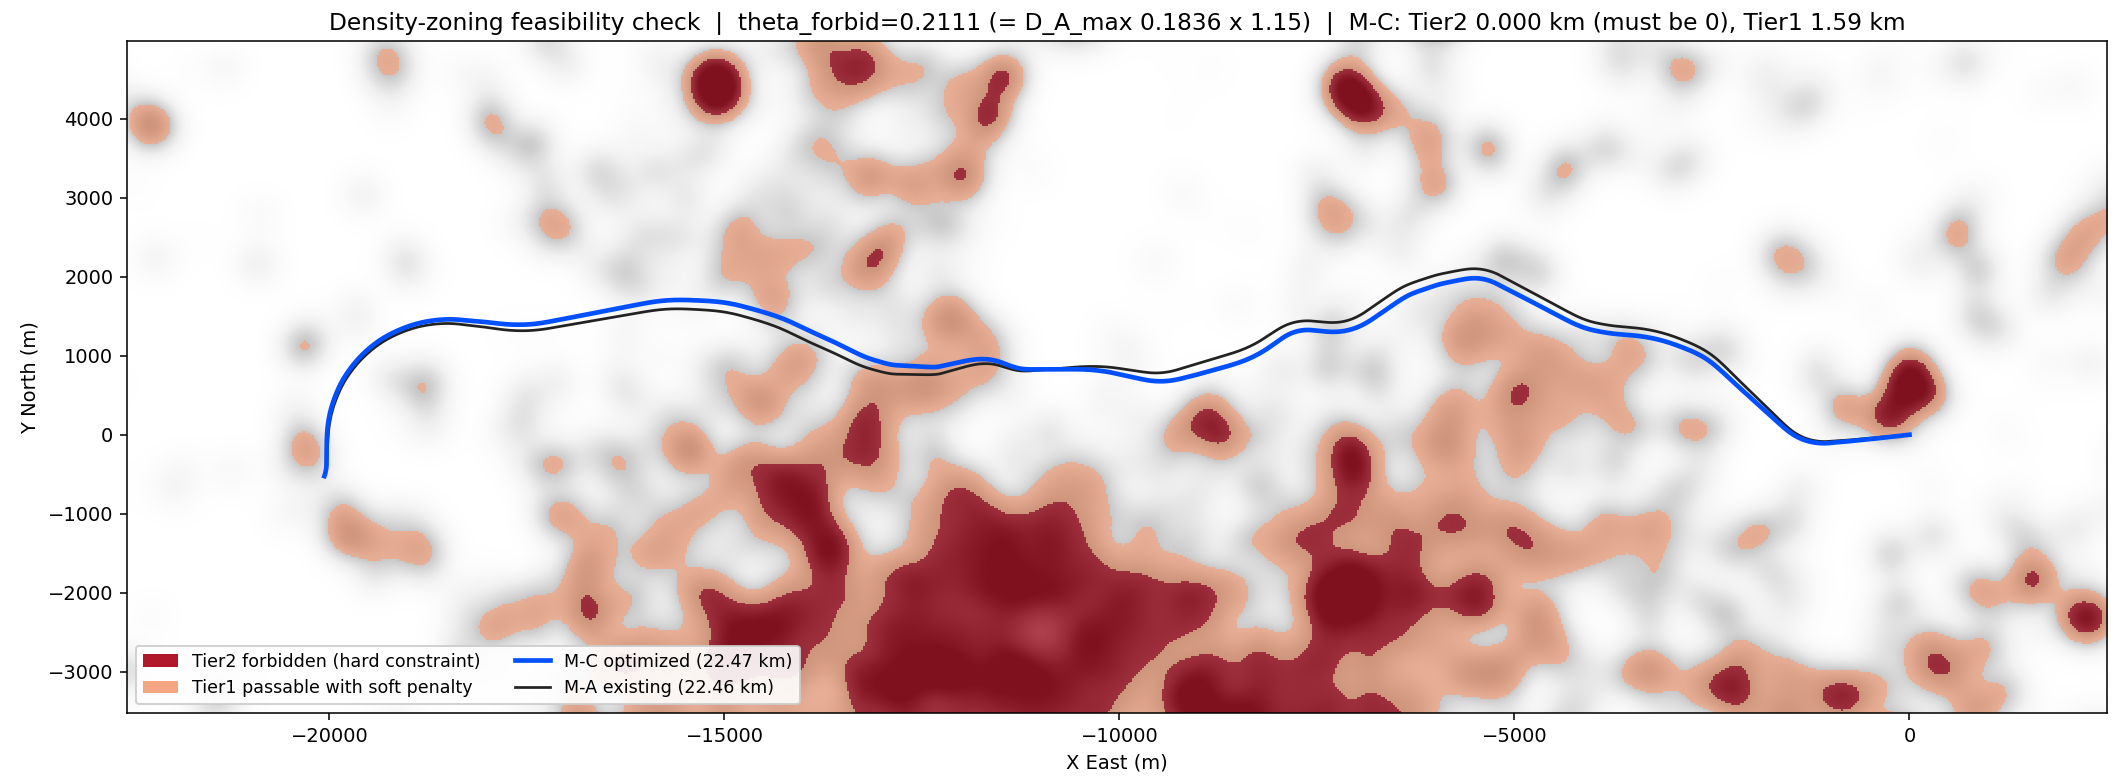
\includegraphics[width=\textwidth]{density_feasibility_w500.png}
\caption{建筑密度分区可行性核验：M-C完全绕避Tier 2，并将Tier 1穿越降至1.59 km。}
\label{fig:density_zh}
\end{figure*}

图\ref{fig:pareto_zh}的可行前沿含少量高造价、低能耗结构化端点。预算约束与非支配筛选先剔除极端方案，熵权仅在工程可接受前沿中选点，避免全局极差归一化偏向病态端点。

\begin{figure}[t]
\centering

\includegraphics[width=\linewidth]{current_pareto_density.pdf}
\caption{当前端点/密度约束下的可行与非支配解筛选。}
\label{fig:pareto_zh}
\end{figure}

图\ref{fig:3d_zh}从空间上区分常规路基、OSM触发桥和生态隧道。当前M-C含约4.08 km跨越桥与0.75 km白云山生态隧道；这些数字直接来自密度约束结果，而非仓库中旧C11图的4.91/0.18 km。

\begin{figure*}[t]
\centering

\includegraphics[width=\textwidth]{current_alignment_3d.pdf}
\caption{当前M-C在准天然DEM上的三维线形，虚线为M-A现状中线。}
\label{fig:3d_zh}
\end{figure*}
\FloatBarrier

\subsection{历史密度前控制：探索性证据}

该控制在端点锚定与建筑分区加入前完成。两阶段方案$C=23.1582$亿元、$E=13.4569$亿元，表面优于联合方案的24.2239/13.4766亿元；但其$R_{min}=397$ m、罚值$7.36\times10^{-2}$，而联合方案$R_{min}=401$ m、罚值为0。它揭示冻结平面后的历史失效模式，但必须在当前端点/密度模型上重跑后才能量化协同效应。

\subsection{历史同代数IJS消融}

表\ref{tab:ablation_zh}给出30次历史运行。同代数下IJS均值由0.9133降至0.6808，并在187代达到JS第500代水平；但25.45\%差距同时包含约3倍NFE与旧自由端点目标，不能解释为等预算提升。DE的观察差距最大（24.17\%）但也使NFE加倍。表中未校正秩和$p$值仅用于审计，不作确认性推断。

\begin{table}[t]
\centering
\caption{历史同代数消融；各变体NFE不同，$p$为未校正独立样本秩和检验。}
\label{tab:ablation_zh}
\begin{tabular}{lrrrrr}
\toprule
变体 & 平均$F$ & 标准差 & $F_{100}$ & 较JS改善 & $p$ \\
\midrule
JS & 0.9133 & 0.0637 & 2.547 & -- & -- \\
JS+Tent & 0.8989 & 0.0605 & 2.227 & 1.58\% & 0.464 \\
JS+L\'evy & 0.8787 & 0.0558 & 2.095 & 3.79\% & 0.0555 \\
JS+DE & 0.6926 & 0.0315 & 1.679 & 24.17\% & $3.02\times10^{-11}$ \\
IJS & \textbf{0.6808} & 0.0340 & \textbf{1.292} & \textbf{25.45\%} & $3.02\times10^{-11}$ \\
\bottomrule
\end{tabular}
\end{table}

\begin{figure*}[t]
\centering
\begin{subfigure}{.48\textwidth}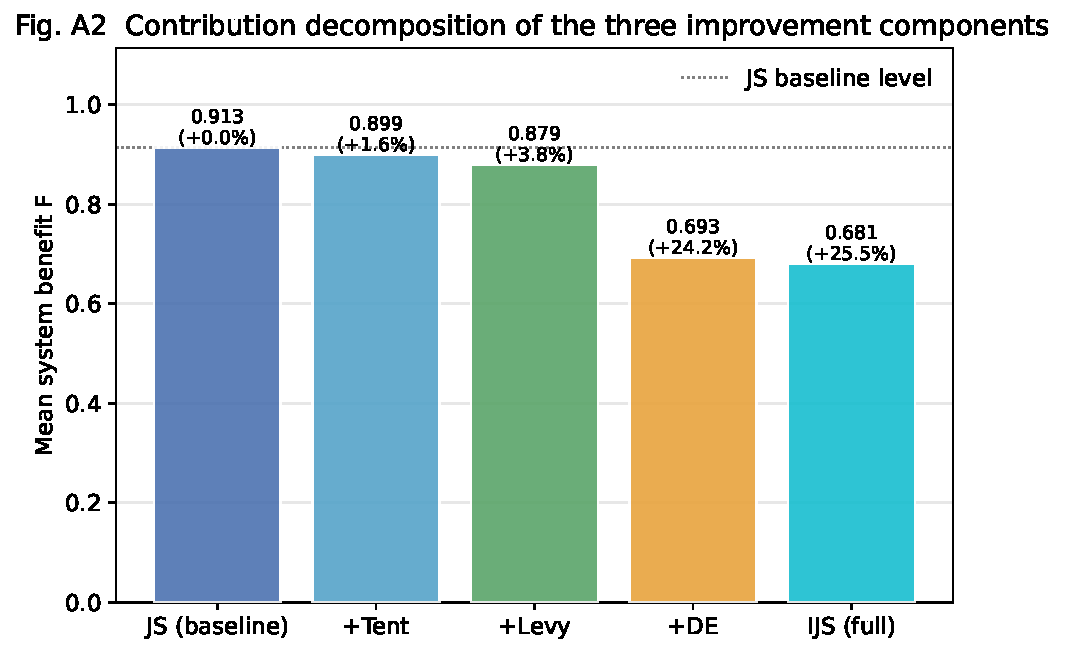
\includegraphics[width=\linewidth]{ablation_contributions.pdf}\caption{组件贡献。}\end{subfigure}\hfill
\begin{subfigure}{.48\textwidth}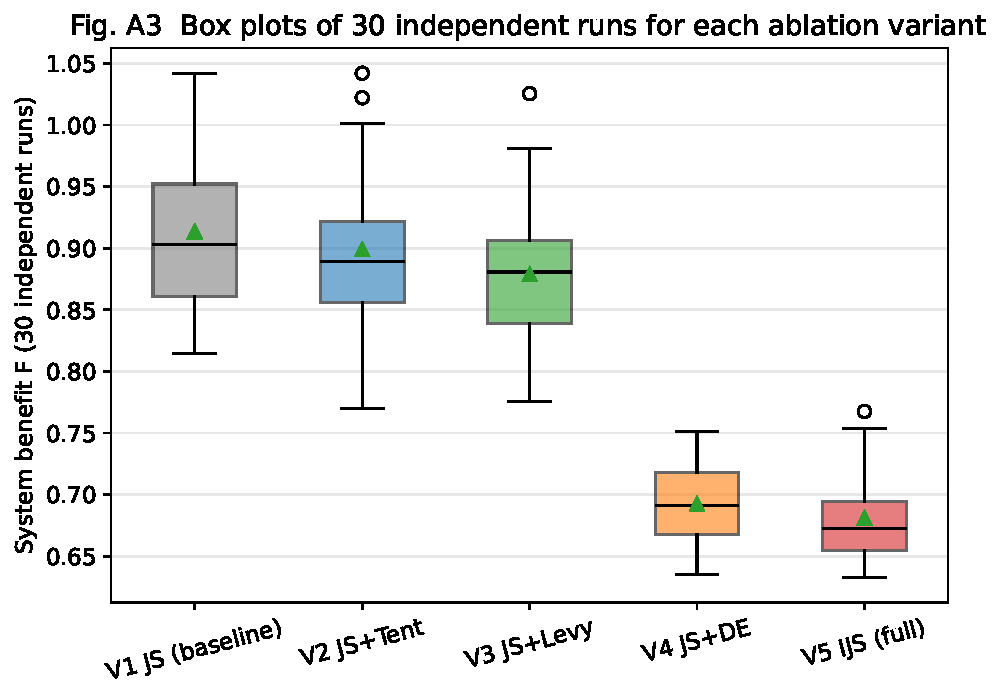
\includegraphics[width=\linewidth]{ablation_boxplot.pdf}\caption{运行分布。}\end{subfigure}
\caption{IJS消融结果，$F$越低越优。}
\end{figure*}
\FloatBarrier

机制插桩显示，独立Tent链替换了200个初始个体中的132个；DE在末100代仍贡献约0.018的$F$下降，说明其不仅是早期加速，还承担后期精修。完整IJS几乎没有持续20代停滞，因此预设“停滞后逃逸率”指标不适用，不能将其机械记为0并解释为L\'evy无效。

\subsection{历史同代数多算法对比}

同代数下IJS在六个历史规模上均有最低平均$F$（表\ref{tab:bench_zh}），但旧模型端点自由且IJS每代约3倍NFE，故不能据此证明等预算优越。PJ6中IJS和JS可行率10/10，其余四种为0/10；该现象只能作为当前模型等NFE复现实验的待检验假设。

\begin{table*}[t]
\centering
\caption{历史十次运行$F$均值（标准差）；同代数不等于同NFE。}
\label{tab:bench_zh}
\scriptsize
\resizebox{\textwidth}{!}{\begin{tabular}{lrrrrrr}
\toprule
算法 & PJ1（95） & PJ2 & PJ3 & PJ4 & PJ5 & PJ6（500） \\
\midrule
IJS & \textbf{.6617 (.0051)} & \textbf{.5986 (.0045)} & \textbf{.7087 (.0045)} & \textbf{.7090 (.0033)} & \textbf{.7778 (.0078)} & \textbf{.8333 (.0019)} \\
JS & .6771 (.0052) & .6104 (.0049) & .7237 (.0063) & .7215 (.0066) & .7954 (.0020) & .8563 (.0060) \\
NSGA-II & .6792 (.0045) & .6240 (.0057) & .7282 (.0053) & .7287 (.0080) & .8104 (.0084) & 12.8859 (.7330) \\
GA & .7103 (.0088) & .6478 (.0171) & .7515 (.0090) & .7489 (.0071) & 5.3906 (.5481) & 25.6024 (1.0630) \\
PSO & .7023 (.0116) & .6370 (.0113) & .7436 (.0070) & .7632 (.0072) & 9.1988 (.9109) & 32.7437 (.6336) \\
GWO & .6843 (.0065) & .6194 (.0070) & .7233 (.0046) & .7276 (.0070) & 1.1104 (.0158) & 3.2157 (1.5706) \\
\bottomrule
\end{tabular}}
\end{table*}

\begin{figure*}[t]
\centering
\begin{subfigure}{.64\textwidth}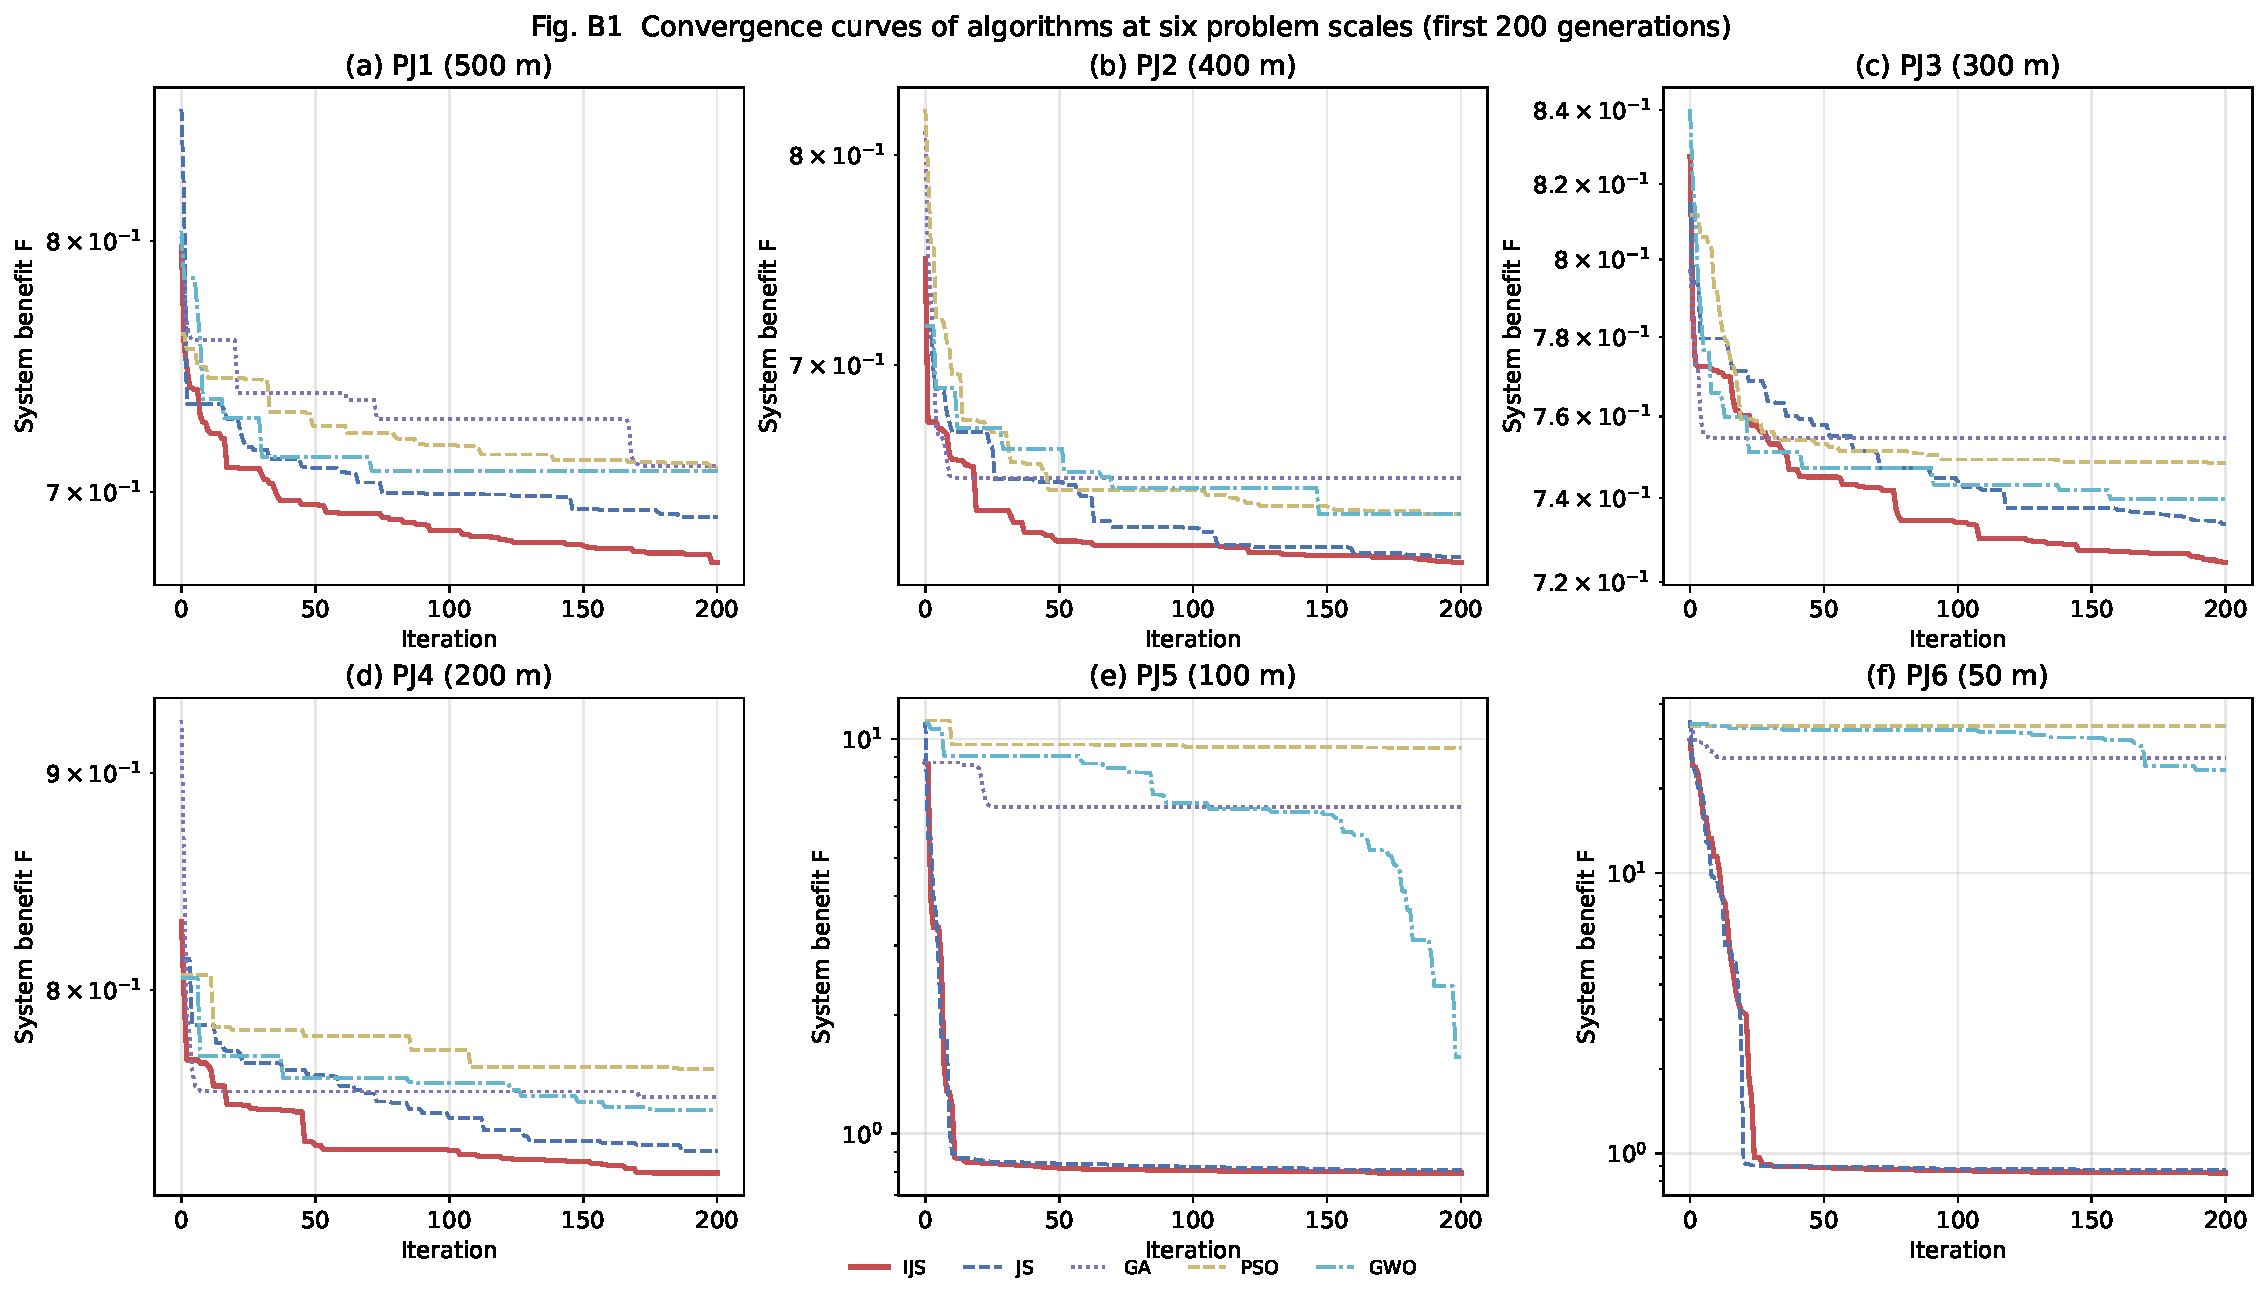
\includegraphics[width=\linewidth]{algorithm_convergence.pdf}\caption{六规模收敛。}\end{subfigure}\hfill
\begin{subfigure}{.33\textwidth}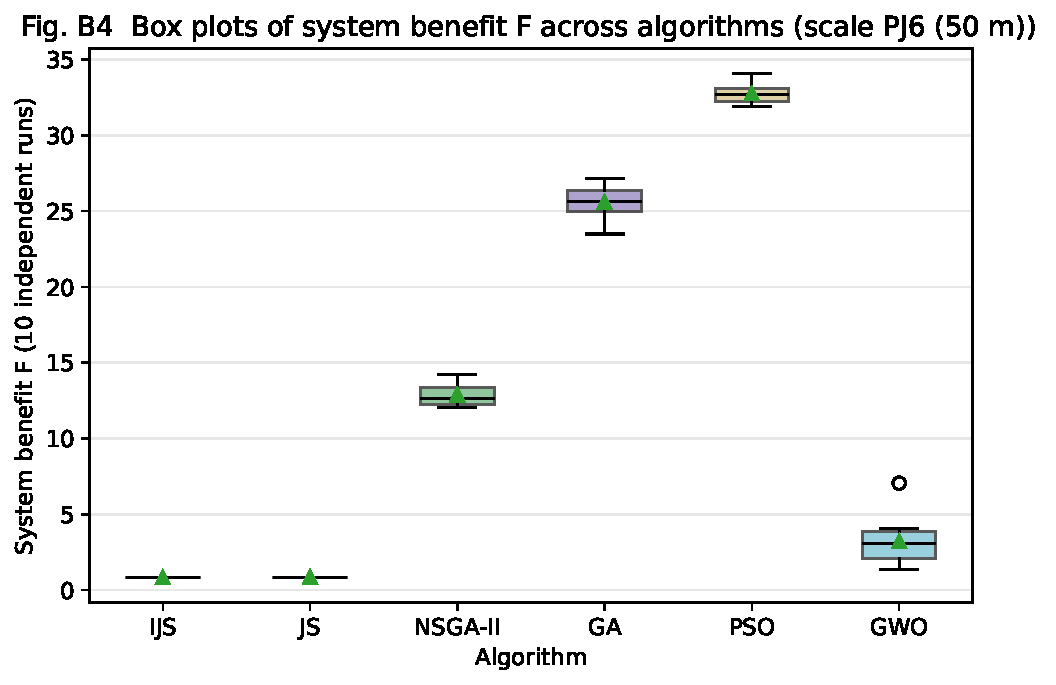
\includegraphics[width=\linewidth]{algorithm_pj6_boxplot.pdf}\caption{PJ6分布。}\end{subfigure}
\caption{历史同代数多算法对比；IJS每代约3倍种群NFE，本图仅作描述。}
\end{figure*}
\FloatBarrier

IJS在PJ1--PJ5耗时约为单阶段算法2倍。现有记录只支持“每代更多求值时历史$F$更低”；当前模型必须按目标调用上限停止，预注册配对种子，并报告多重校正、效应量、置信区间和时间。

\subsection{历史自由端点重优化敏感性}

历史自由端点模型的237个敏感性点全部可行，但不能验证当前端点/密度模型稳健性。该旧模型中，交通增长对能耗影响最大；基础设施成本在建设期发生，因而对交通、渗透率和能源价格相对稳定。提高电动车渗透率可缓解高增长情景的能耗负担，油电价格同步增长则显著抬升货币化$E$。

走廊带半宽表现出先快速、后饱和的降本规律：匹配重优化实验中，200 m时$C=25.68$亿元，2,500 m时降至22.39亿元；线位具备绕离生态隧道区的空间后，边际收益逐步受城市与曲率约束限制。桥梁两端延伸$E_{ext}=50/75/100$ m时，$C$分别为22.81/23.55/24.74亿元，而$E$保持约13.55亿元，表明该不确定工程参数主要平移结构成本，不改变能耗结论。

\begin{figure*}[t]
\centering
\begin{subfigure}{.48\textwidth}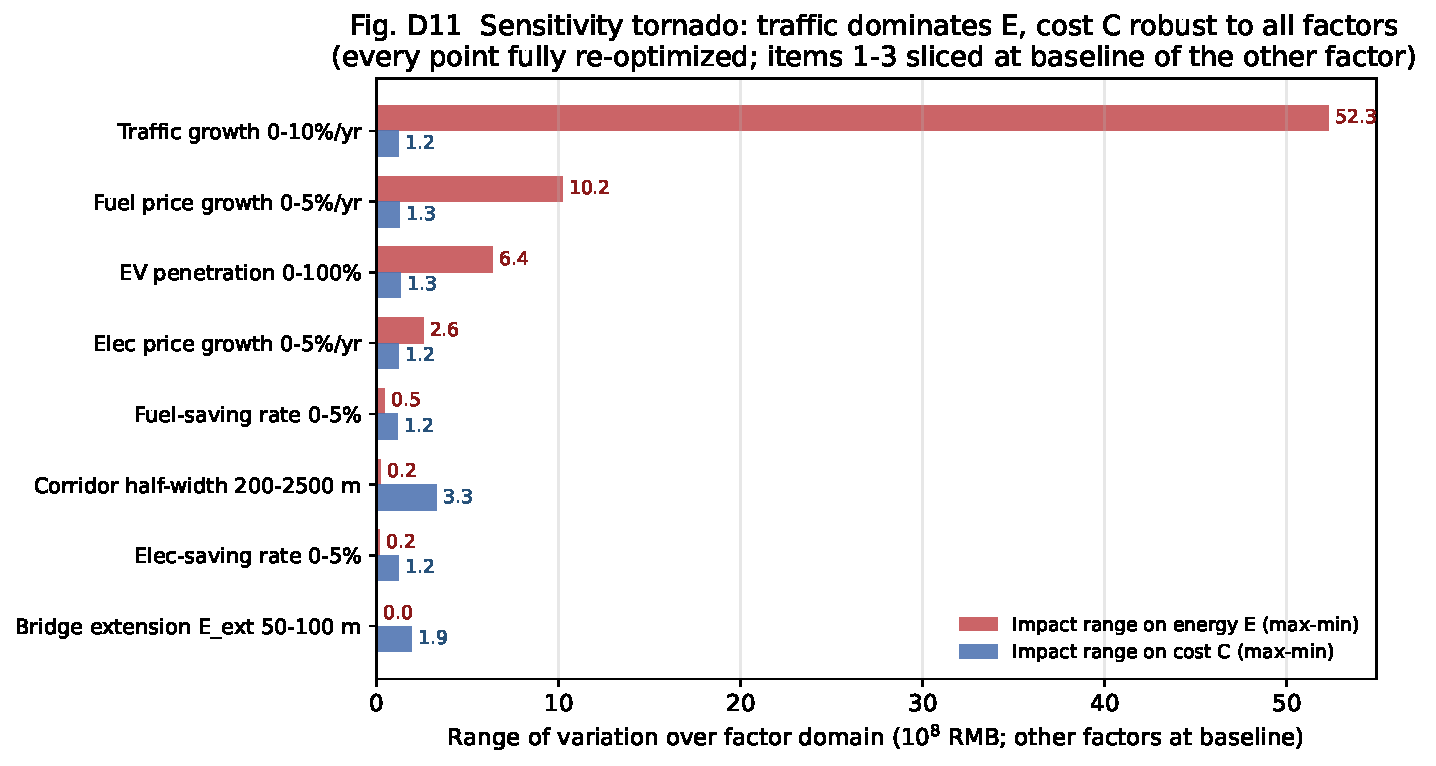
\includegraphics[width=\linewidth]{sensitivity_tornado.pdf}\caption{因素重要性。}\end{subfigure}\hfill
\begin{subfigure}{.48\textwidth}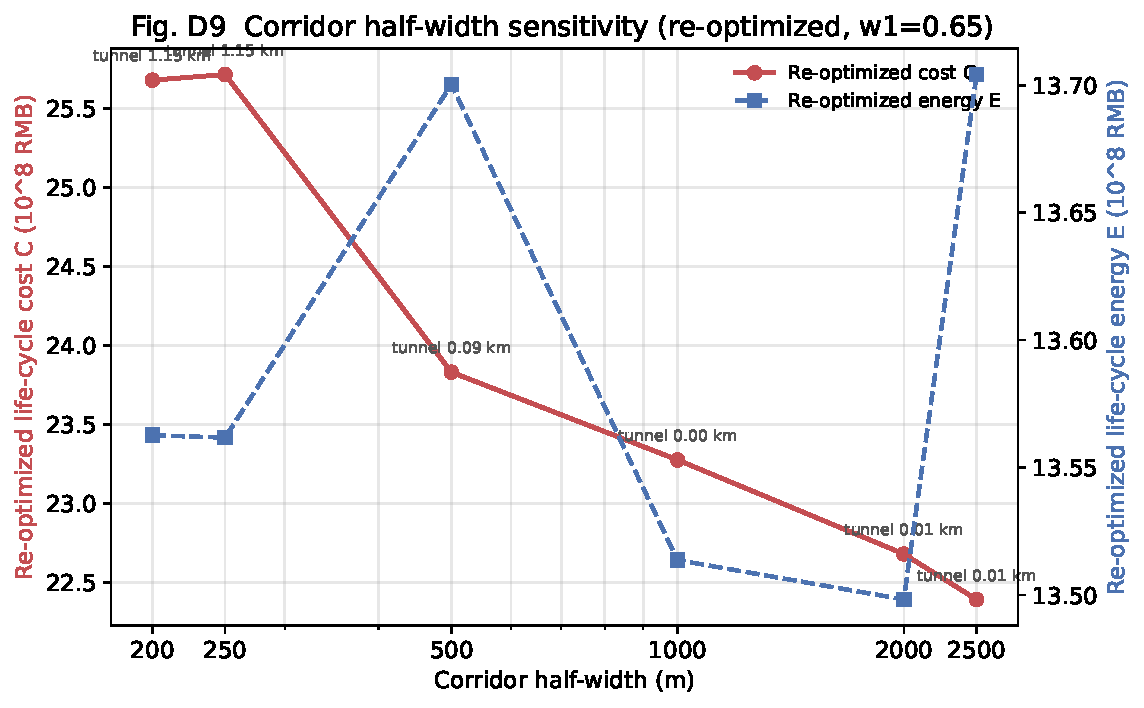
\includegraphics[width=\linewidth]{corridor_sensitivity.pdf}\caption{走廊带重优化。}\end{subfigure}
\caption{历史自由端点敏感性；每个点均重优化，但实验早于端点锚定与密度分区。}
\end{figure*}
\FloatBarrier

\section{讨论}

\subsection{降本节能的工程解释}

8.33\%是本案例、共同单价和共同数据下的相对变化，不能外推为所有高速公路的固定节省率。其可信性来自分项机制：M-C略长且土方更多，但桥隧和运行能耗下降，并完全绕开Tier 2。优化器在真实分项间进行交换，而不是单纯靠缩短里程。端点高程锚定进一步排除了不可接线纵断面的虚假节能。

两阶段控制说明，低目标值不是充分证据。397 m半径使其不具备可比资格。联合搜索保留了移动平面交叉位置与调整纵断面的自由度，尤其适用于跨越桥与坡度过渡相互作用的路段。

\subsection{DEM/OSM与算法创新的作用}

DEM使每条候选平面线位重新采样地面；若仍按原中线比例取高程，横移只能改变里程，平纵联合的主要土方通道被结构性抹除。OSM则把跨越结构和城市暴露与几何相交联系起来。该模型仍不等同于勘察设计：它缺乏桥面高程、地块权属和完整建筑属性，但已将早期走廊优化从一维中线提升为可复核的空间筛选。

历史消融不支持“混沌初始化决定一切”的叙事：Tent观察差距最小、DE最大。但组件开关同时改变NFE，现有证据不能把算子质量与预算分离。Tent覆盖、L\'evy探索和DE精修仍是合理待检验机制；高维可行率优势能否在当前模型等NFE下保持尚未解决。

\subsection{局限性与效度边界}

\begin{enumerate}[leftmargin=*,label=(\arabic*)]
\item 准天然DEM由现状道路影响带重建，并非建路前实测；8.8 m像元不能表达局部排水、挡墙和微地形。
\item OSM完整性不均。secondary道路不触发桥；缺少被交设施结构高程，暂不能实施竖向净空；15°交角按现状最小15.6°校准。
\item Tier-1权重0.22属于规划抑制项，不是实测拆迁费用。早期消融、算法对比和敏感性同时采用密度前、自由端点目标且NFE不等，仅是探索性开发记录。
\item 能耗目标为货币量且只计算代表方向。端点锚定解决净落差套利，但最终设计需要双向交通加权和经标定的再生制动。
\item 相邻坡差只是竖曲线代理；尚未显式实施凸/凹竖曲线长度、不重叠、视距、缓和曲线/圆曲线分段和完整平纵组合约束。
\item 造价为前期估算口径，地质、水文、地块权属、施工组织、隐含碳和概率不确定性尚未进入模型。
\item 当前密度约束主方案仅一次优化。需补充多种子复现；算法结论还需等NFE、多重校正、效应量与置信区间。存储向量中一个旧起点基因不活跃，也应在下次实验删除。
\end{enumerate}

因此本文结论适用于可复现的走廊级决策与方法比较，不能直接替代详细路线和施工图设计。

\section{结论}

本文提出将三维几何、全生命周期成本和油电混行能耗联系起来的高速公路平纵协同优化方法。在既有数学模型基础上，进一步引入准天然DEM、OSM交叉桥、生态隧道、建筑密度分区、结构替代和接线端点锚定，并以IJS和“先可行、再非支配、后熵权”流程求解。

广州北环高速当前$W=500$ m密度约束方案实现成本降低8.33\%、货币化能耗降低3.00\%，最小半径421 m、硬罚为0、Tier 2穿越为0。线位略长且土方增加，说明净收益来自可解释的结构与运行权衡。历史两阶段控制表明，不可行的更低目标不能替代协同可行解；早期消融、算法对比和敏感性可记录模型开发路径，但其自由端点口径和不等NFE不能验证当前模型。当前算法结论必须以等预算、多种子复现为前提。

后续应优先补充双向能耗、测量级障碍物高程、显式竖曲线与视距、地块/隐含碳目标、造价不确定性，以及最新密度方案的多种子统计，从走廊级智能比选进一步迈向设计级决策支持。

\section*{数据与代码可用性}
论文由RoadPlan实验仓库生成。GNSS及项目派生文件可能受数据所有者限制；处理后的DEM/OSM、源代码、固定随机种子、结果JSON和制图脚本已按复现逻辑组织。双盲审稿后应补充公开仓库与DOI（当前为数据仓库DOI占位符）。

\section*{作者贡献}
\textbf{[作者姓名占位]}：概念设计、方法、软件、验证、调查、数据整理、可视化、初稿、审阅与修改。投稿前须按真实分工替换。

\section*{利益冲突声明}
作者声明不存在可能影响本文工作的已知经济利益或个人关系；投稿前须由全部作者确认。

\section*{致谢}
基金名称、编号及非作者贡献因双盲审稿暂作匿名占位，投稿前补全。

\bibliographystyle{elsarticle-num}
\bibliography{../references}

\end{document}
